% !TEX TS-program = pdflatex
% !TEX encoding = UTF-8 Unicode
\documentclass[border=0mm]{standalone}
% packages
\usepackage{tikz}
\usetikzlibrary{patterns}
\usepackage{amsmath,amssymb}
\usepackage{bm}
\usepackage{pgfplots}
\pgfplotsset{compat=1.15}
% start document
\begin{document}
% generated by ROOT (CERN)
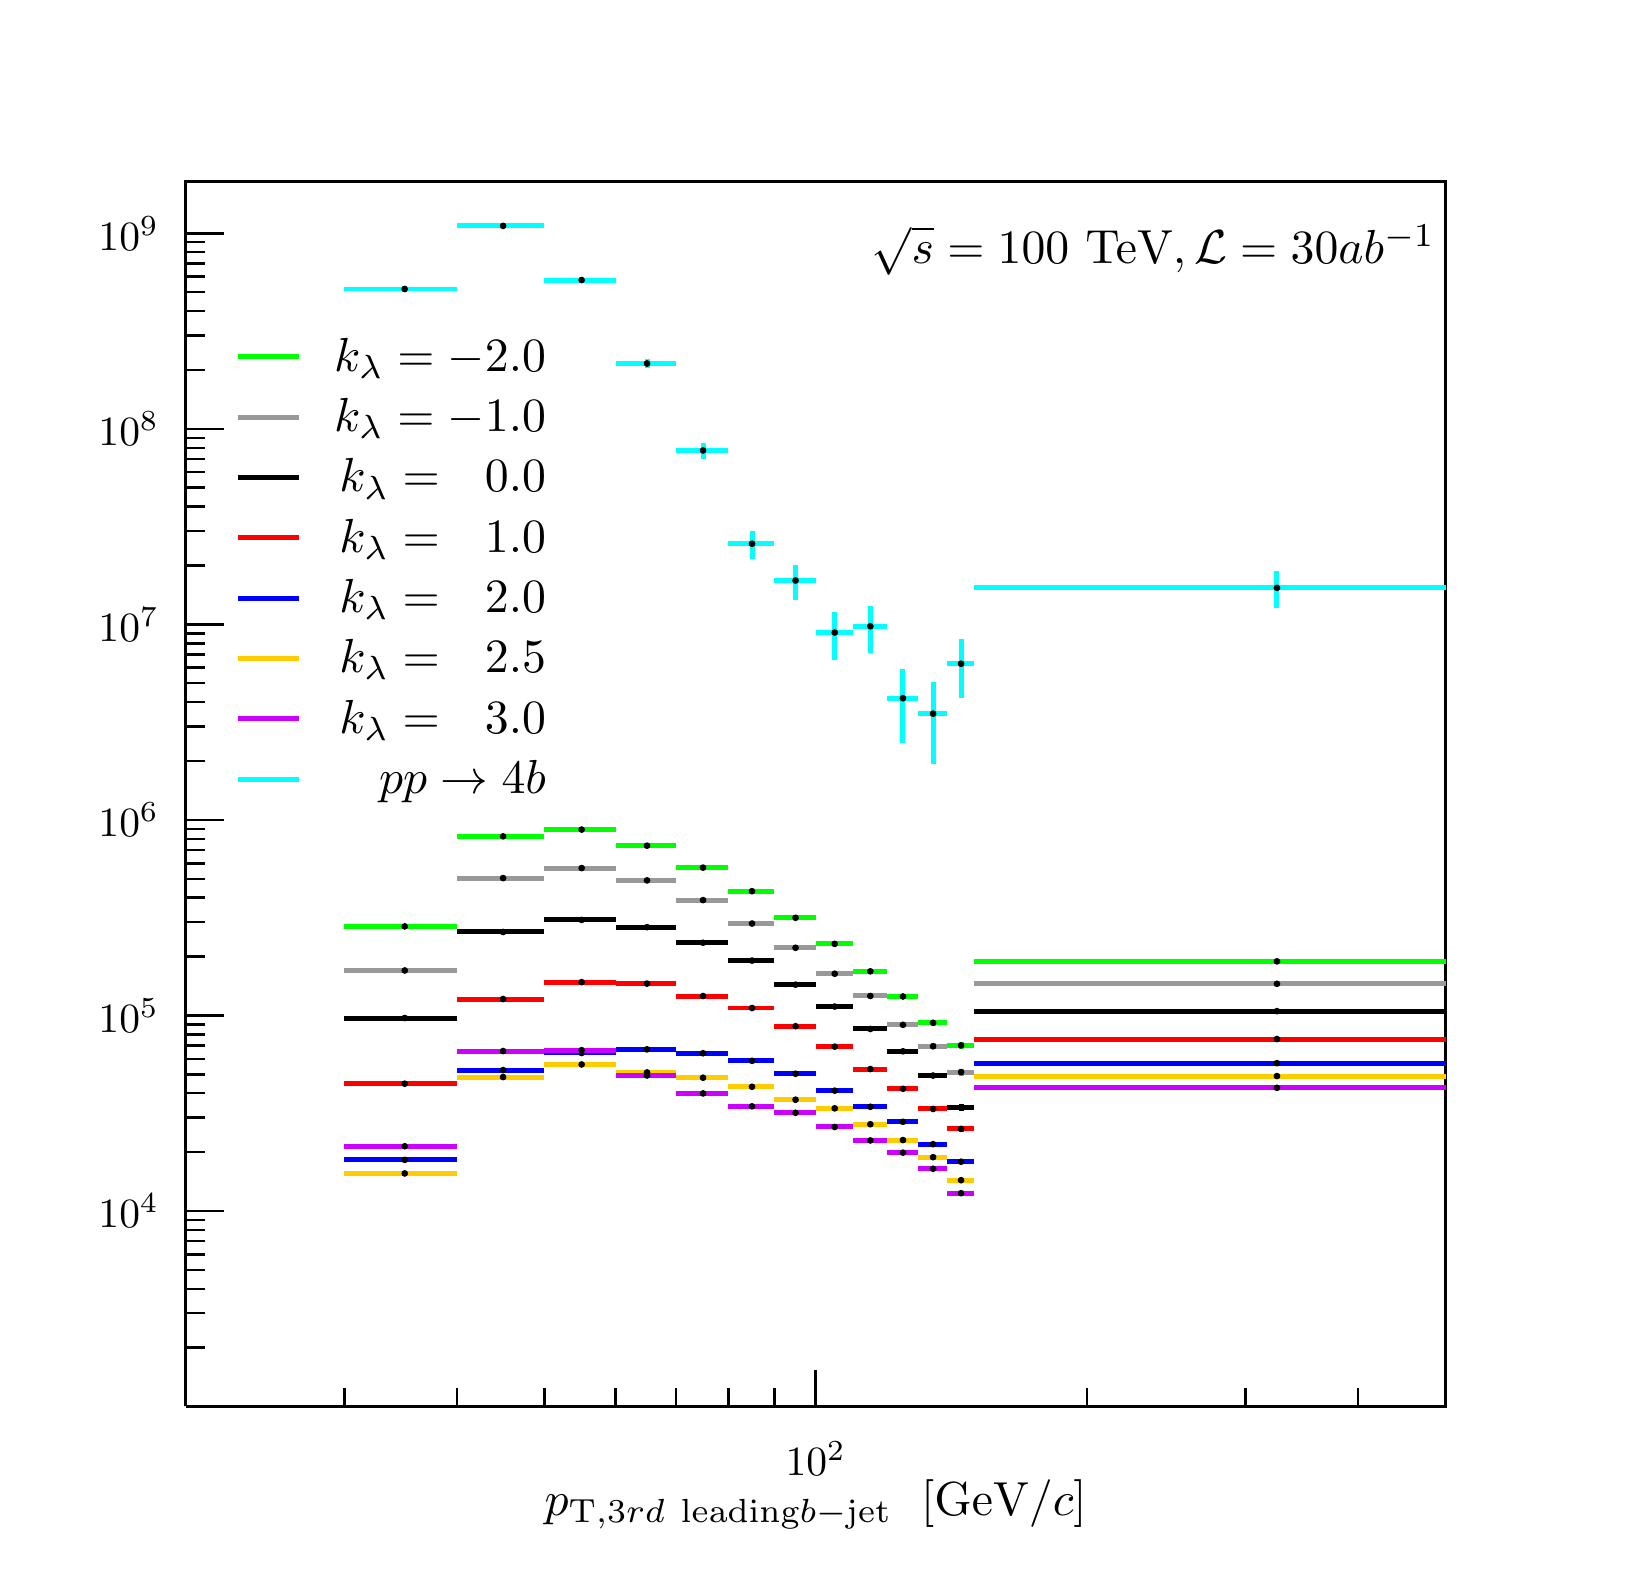
\begin{tikzpicture}
\pgfdeclareplotmark{cross} {
\pgfpathmoveto{\pgfpoint{-0.3\pgfplotmarksize}{\pgfplotmarksize}}
\pgfpathlineto{\pgfpoint{+0.3\pgfplotmarksize}{\pgfplotmarksize}}
\pgfpathlineto{\pgfpoint{+0.3\pgfplotmarksize}{0.3\pgfplotmarksize}}
\pgfpathlineto{\pgfpoint{+1\pgfplotmarksize}{0.3\pgfplotmarksize}}
\pgfpathlineto{\pgfpoint{+1\pgfplotmarksize}{-0.3\pgfplotmarksize}}
\pgfpathlineto{\pgfpoint{+0.3\pgfplotmarksize}{-0.3\pgfplotmarksize}}
\pgfpathlineto{\pgfpoint{+0.3\pgfplotmarksize}{-1.\pgfplotmarksize}}
\pgfpathlineto{\pgfpoint{-0.3\pgfplotmarksize}{-1.\pgfplotmarksize}}
\pgfpathlineto{\pgfpoint{-0.3\pgfplotmarksize}{-0.3\pgfplotmarksize}}
\pgfpathlineto{\pgfpoint{-1.\pgfplotmarksize}{-0.3\pgfplotmarksize}}
\pgfpathlineto{\pgfpoint{-1.\pgfplotmarksize}{0.3\pgfplotmarksize}}
\pgfpathlineto{\pgfpoint{-0.3\pgfplotmarksize}{0.3\pgfplotmarksize}}
\pgfpathclose
\pgfusepathqstroke
}
\pgfdeclareplotmark{cross*} {
\pgfpathmoveto{\pgfpoint{-0.3\pgfplotmarksize}{\pgfplotmarksize}}
\pgfpathlineto{\pgfpoint{+0.3\pgfplotmarksize}{\pgfplotmarksize}}
\pgfpathlineto{\pgfpoint{+0.3\pgfplotmarksize}{0.3\pgfplotmarksize}}
\pgfpathlineto{\pgfpoint{+1\pgfplotmarksize}{0.3\pgfplotmarksize}}
\pgfpathlineto{\pgfpoint{+1\pgfplotmarksize}{-0.3\pgfplotmarksize}}
\pgfpathlineto{\pgfpoint{+0.3\pgfplotmarksize}{-0.3\pgfplotmarksize}}
\pgfpathlineto{\pgfpoint{+0.3\pgfplotmarksize}{-1.\pgfplotmarksize}}
\pgfpathlineto{\pgfpoint{-0.3\pgfplotmarksize}{-1.\pgfplotmarksize}}
\pgfpathlineto{\pgfpoint{-0.3\pgfplotmarksize}{-0.3\pgfplotmarksize}}
\pgfpathlineto{\pgfpoint{-1.\pgfplotmarksize}{-0.3\pgfplotmarksize}}
\pgfpathlineto{\pgfpoint{-1.\pgfplotmarksize}{0.3\pgfplotmarksize}}
\pgfpathlineto{\pgfpoint{-0.3\pgfplotmarksize}{0.3\pgfplotmarksize}}
\pgfpathclose
\pgfusepathqfillstroke
}
\pgfdeclareplotmark{newstar} {
\pgfpathmoveto{\pgfqpoint{0pt}{\pgfplotmarksize}}
\pgfpathlineto{\pgfqpointpolar{44}{0.5\pgfplotmarksize}}
\pgfpathlineto{\pgfqpointpolar{18}{\pgfplotmarksize}}
\pgfpathlineto{\pgfqpointpolar{-20}{0.5\pgfplotmarksize}}
\pgfpathlineto{\pgfqpointpolar{-54}{\pgfplotmarksize}}
\pgfpathlineto{\pgfqpointpolar{-90}{0.5\pgfplotmarksize}}
\pgfpathlineto{\pgfqpointpolar{234}{\pgfplotmarksize}}
\pgfpathlineto{\pgfqpointpolar{198}{0.5\pgfplotmarksize}}
\pgfpathlineto{\pgfqpointpolar{162}{\pgfplotmarksize}}
\pgfpathlineto{\pgfqpointpolar{134}{0.5\pgfplotmarksize}}
\pgfpathclose
\pgfusepathqstroke
}
\pgfdeclareplotmark{newstar*} {
\pgfpathmoveto{\pgfqpoint{0pt}{\pgfplotmarksize}}
\pgfpathlineto{\pgfqpointpolar{44}{0.5\pgfplotmarksize}}
\pgfpathlineto{\pgfqpointpolar{18}{\pgfplotmarksize}}
\pgfpathlineto{\pgfqpointpolar{-20}{0.5\pgfplotmarksize}}
\pgfpathlineto{\pgfqpointpolar{-54}{\pgfplotmarksize}}
\pgfpathlineto{\pgfqpointpolar{-90}{0.5\pgfplotmarksize}}
\pgfpathlineto{\pgfqpointpolar{234}{\pgfplotmarksize}}
\pgfpathlineto{\pgfqpointpolar{198}{0.5\pgfplotmarksize}}
\pgfpathlineto{\pgfqpointpolar{162}{\pgfplotmarksize}}
\pgfpathlineto{\pgfqpointpolar{134}{0.5\pgfplotmarksize}}
\pgfpathclose
\pgfusepathqfillstroke
}
\definecolor{c}{rgb}{1,1,1};
\draw [color=c, fill=c] (0,0) rectangle (20,19.4486);
\draw [color=c, fill=c] (0,0) rectangle (20,19.4486);
\draw [color=c, fill=c] (2,1.94486) rectangle (18,17.5038);
\definecolor{c}{rgb}{0,0,0};
\draw [c,line width=0.9] (2,1.94486) -- (2,17.5038) -- (18,17.5038) -- (18,1.94486) -- (2,1.94486);
\definecolor{c}{rgb}{1,1,1};
\draw [color=c, fill=c] (2,1.94486) rectangle (18,17.5038);
\definecolor{c}{rgb}{0,0,0};
\draw [c,line width=0.9] (2,1.94486) -- (2,17.5038) -- (18,17.5038) -- (18,1.94486) -- (2,1.94486);
\definecolor{c}{rgb}{0,1,1};
\draw [c,line width=1.8] (4.78167,16.0963) -- (4.78167,16.1366);
\draw [c,line width=1.8] (4.78167,16.1366) -- (4.78167,16.1754);
\draw [c,line width=1.8] (4.01544,16.1366) -- (4.78167,16.1366);
\draw [c,line width=1.8] (4.78167,16.1366) -- (5.44541,16.1366);
\definecolor{c}{rgb}{0,0,0};
\foreach \P in {(4.78167,16.1366)}{\draw[mark options={color=c,fill=c},mark size=2.402402pt,mark=*,mark size=1pt] plot coordinates {\P};}
\definecolor{c}{rgb}{0,1,1};
\draw [c,line width=1.8] (6.03087,16.9102) -- (6.03087,16.9379);
\draw [c,line width=1.8] (6.03087,16.9379) -- (6.03087,16.9648);
\draw [c,line width=1.8] (5.44541,16.9379) -- (6.03087,16.9379);
\draw [c,line width=1.8] (6.03087,16.9379) -- (6.55459,16.9379);
\definecolor{c}{rgb}{0,0,0};
\foreach \P in {(6.03087,16.9379)}{\draw[mark options={color=c,fill=c},mark size=2.402402pt,mark=*,mark size=1pt] plot coordinates {\P};}
\definecolor{c}{rgb}{0,1,1};
\draw [c,line width=1.8] (7.02834,16.2113) -- (7.02834,16.2495);
\draw [c,line width=1.8] (7.02834,16.2495) -- (7.02834,16.2864);
\draw [c,line width=1.8] (6.55459,16.2495) -- (7.02834,16.2495);
\draw [c,line width=1.8] (7.02834,16.2495) -- (7.46085,16.2495);
\definecolor{c}{rgb}{0,0,0};
\foreach \P in {(7.02834,16.2495)}{\draw[mark options={color=c,fill=c},mark size=2.402402pt,mark=*,mark size=1pt] plot coordinates {\P};}
\definecolor{c}{rgb}{0,1,1};
\draw [c,line width=1.8] (7.85872,15.1272) -- (7.85872,15.1904);
\draw [c,line width=1.8] (7.85872,15.1904) -- (7.85872,15.2501);
\draw [c,line width=1.8] (7.46085,15.1904) -- (7.85872,15.1904);
\draw [c,line width=1.8] (7.85872,15.1904) -- (8.22708,15.1904);
\definecolor{c}{rgb}{0,0,0};
\foreach \P in {(7.85872,15.1904)}{\draw[mark options={color=c,fill=c},mark size=2.402402pt,mark=*,mark size=1pt] plot coordinates {\P};}
\definecolor{c}{rgb}{0,1,1};
\draw [c,line width=1.8] (8.57002,13.9788) -- (8.57002,14.0863);
\draw [c,line width=1.8] (8.57002,14.0863) -- (8.57002,14.1841);
\draw [c,line width=1.8] (8.22708,14.0863) -- (8.57002,14.0863);
\draw [c,line width=1.8] (8.57002,14.0863) -- (8.89083,14.0863);
\definecolor{c}{rgb}{0,0,0};
\foreach \P in {(8.57002,14.0863)}{\draw[mark options={color=c,fill=c},mark size=2.402402pt,mark=*,mark size=1pt] plot coordinates {\P};}
\definecolor{c}{rgb}{0,1,1};
\draw [c,line width=1.8] (9.19217,12.7078) -- (9.19217,12.9015);
\draw [c,line width=1.8] (9.19217,12.9015) -- (9.19217,13.0657);
\draw [c,line width=1.8] (8.89083,12.9015) -- (9.19217,12.9015);
\draw [c,line width=1.8] (9.19217,12.9015) -- (9.47629,12.9015);
\definecolor{c}{rgb}{0,0,0};
\foreach \P in {(9.19217,12.9015)}{\draw[mark options={color=c,fill=c},mark size=2.402402pt,mark=*,mark size=1pt] plot coordinates {\P};}
\definecolor{c}{rgb}{0,1,1};
\draw [c,line width=1.8] (9.74504,12.1885) -- (9.74504,12.4347);
\draw [c,line width=1.8] (9.74504,12.4347) -- (9.74504,12.635);
\draw [c,line width=1.8] (9.47629,12.4347) -- (9.74504,12.4347);
\draw [c,line width=1.8] (9.74504,12.4347) -- (10,12.4347);
\definecolor{c}{rgb}{0,0,0};
\foreach \P in {(9.74504,12.4347)}{\draw[mark options={color=c,fill=c},mark size=2.402402pt,mark=*,mark size=1pt] plot coordinates {\P};}
\definecolor{c}{rgb}{0,1,1};
\draw [c,line width=1.8] (10.2425,11.4232) -- (10.2425,11.7735);
\draw [c,line width=1.8] (10.2425,11.7735) -- (10.2425,12.0375);
\draw [c,line width=1.8] (10,11.7735) -- (10.2425,11.7735);
\draw [c,line width=1.8] (10.2425,11.7735) -- (10.4738,11.7735);
\definecolor{c}{rgb}{0,0,0};
\foreach \P in {(10.2425,11.7735)}{\draw[mark options={color=c,fill=c},mark size=2.402402pt,mark=*,mark size=1pt] plot coordinates {\P};}
\definecolor{c}{rgb}{0,1,1};
\draw [c,line width=1.8] (10.6947,11.5181) -- (10.6947,11.8534);
\draw [c,line width=1.8] (10.6947,11.8534) -- (10.6947,12.1089);
\draw [c,line width=1.8] (10.4738,11.8534) -- (10.6947,11.8534);
\draw [c,line width=1.8] (10.6947,11.8534) -- (10.9063,11.8534);
\definecolor{c}{rgb}{0,0,0};
\foreach \P in {(10.6947,11.8534)}{\draw[mark options={color=c,fill=c},mark size=2.402402pt,mark=*,mark size=1pt] plot coordinates {\P};}
\definecolor{c}{rgb}{0,1,1};
\draw [c,line width=1.8] (11.1092,10.3739) -- (11.1092,10.9397);
\draw [c,line width=1.8] (11.1092,10.9397) -- (11.1092,11.3089);
\draw [c,line width=1.8] (10.9063,10.9397) -- (11.1092,10.9397);
\draw [c,line width=1.8] (11.1092,10.9397) -- (11.3041,10.9397);
\definecolor{c}{rgb}{0,0,0};
\foreach \P in {(11.1092,10.9397)}{\draw[mark options={color=c,fill=c},mark size=2.402402pt,mark=*,mark size=1pt] plot coordinates {\P};}
\definecolor{c}{rgb}{0,1,1};
\draw [c,line width=1.8] (11.4917,10.1038) -- (11.4917,10.7431);
\draw [c,line width=1.8] (11.4917,10.7431) -- (11.4917,11.1417);
\draw [c,line width=1.8] (11.3041,10.7431) -- (11.4917,10.7431);
\draw [c,line width=1.8] (11.4917,10.7431) -- (11.6725,10.7431);
\definecolor{c}{rgb}{0,0,0};
\foreach \P in {(11.4917,10.7431)}{\draw[mark options={color=c,fill=c},mark size=2.402402pt,mark=*,mark size=1pt] plot coordinates {\P};}
\definecolor{c}{rgb}{0,1,1};
\draw [c,line width=1.8] (11.8469,10.9397) -- (11.8469,11.377);
\draw [c,line width=1.8] (11.8469,11.377) -- (11.8469,11.6872);
\draw [c,line width=1.8] (11.6725,11.377) -- (11.8469,11.377);
\draw [c,line width=1.8] (11.8469,11.377) -- (12.0154,11.377);
\definecolor{c}{rgb}{0,0,0};
\foreach \P in {(11.8469,11.377)}{\draw[mark options={color=c,fill=c},mark size=2.402402pt,mark=*,mark size=1pt] plot coordinates {\P};}
\definecolor{c}{rgb}{0,1,1};
\draw [c,line width=1.8] (15.8587,12.0823) -- (15.8587,12.3409);
\draw [c,line width=1.8] (15.8587,12.3409) -- (15.8587,12.5493);
\draw [c,line width=1.8] (12.0154,12.3409) -- (15.8587,12.3409);
\draw [c,line width=1.8] (15.8587,12.3409) -- (18,12.3409);
\definecolor{c}{rgb}{0,0,0};
\foreach \P in {(15.8587,12.3409)}{\draw[mark options={color=c,fill=c},mark size=2.402402pt,mark=*,mark size=1pt] plot coordinates {\P};}
\draw [c,line width=0.9] (2,1.94486) -- (18,1.94486);
\draw [c,line width=0.9] (4.01543,2.17825) -- (4.01543,1.94486);
\draw [c,line width=0.9] (5.4454,2.17825) -- (5.4454,1.94486);
\draw [c,line width=0.9] (6.55458,2.17825) -- (6.55458,1.94486);
\draw [c,line width=0.9] (7.46084,2.17825) -- (7.46084,1.94486);
\draw [c,line width=0.9] (8.22708,2.17825) -- (8.22708,1.94486);
\draw [c,line width=0.9] (8.89082,2.17825) -- (8.89082,1.94486);
\draw [c,line width=0.9] (9.47628,2.17825) -- (9.47628,1.94486);
\draw [c,line width=0.9] (9.99999,2.41163) -- (9.99999,1.94486);
\draw [anchor=base] (9.99999,1.06481) node[scale=1.50291, color=c, rotate=0]{$10^{2}$};
\draw [c,line width=0.9] (13.4454,2.17825) -- (13.4454,1.94486);
\draw [c,line width=0.9] (15.4608,2.17825) -- (15.4608,1.94486);
\draw [c,line width=0.9] (16.8908,2.17825) -- (16.8908,1.94486);
\draw [c,line width=0.9] (18,2.17825) -- (18,1.94486);
\draw (10,0.700151) node[scale=1.72557, color=c, rotate=0]{$ p_{\text{T}, 3rd ~\text{leading} b-\text{jet~}} ~[\text{GeV}/c]$};
\draw [c,line width=0.9] (2,1.94486) -- (2,17.5038);
\draw [c,line width=0.9] (2.24,2.69237) -- (2,2.69237);
\draw [c,line width=0.9] (2.24,3.12964) -- (2,3.12964);
\draw [c,line width=0.9] (2.24,3.43988) -- (2,3.43988);
\draw [c,line width=0.9] (2.24,3.68052) -- (2,3.68052);
\draw [c,line width=0.9] (2.24,3.87715) -- (2,3.87715);
\draw [c,line width=0.9] (2.24,4.04339) -- (2,4.04339);
\draw [c,line width=0.9] (2.24,4.18739) -- (2,4.18739);
\draw [c,line width=0.9] (2.24,4.31441) -- (2,4.31441);
\draw [c,line width=0.9] (2.48,4.42803) -- (2,4.42803);
\draw [anchor= east] (1.844,4.42803) node[scale=1.50291, color=c, rotate=0]{$10^{4}$};
\draw [c,line width=0.9] (2.24,5.17555) -- (2,5.17555);
\draw [c,line width=0.9] (2.24,5.61281) -- (2,5.61281);
\draw [c,line width=0.9] (2.24,5.92306) -- (2,5.92306);
\draw [c,line width=0.9] (2.24,6.1637) -- (2,6.1637);
\draw [c,line width=0.9] (2.24,6.36032) -- (2,6.36032);
\draw [c,line width=0.9] (2.24,6.52656) -- (2,6.52656);
\draw [c,line width=0.9] (2.24,6.67057) -- (2,6.67057);
\draw [c,line width=0.9] (2.24,6.79759) -- (2,6.79759);
\draw [c,line width=0.9] (2.48,6.91121) -- (2,6.91121);
\draw [anchor= east] (1.844,6.91121) node[scale=1.50291, color=c, rotate=0]{$10^{5}$};
\draw [c,line width=0.9] (2.24,7.65872) -- (2,7.65872);
\draw [c,line width=0.9] (2.24,8.09599) -- (2,8.09599);
\draw [c,line width=0.9] (2.24,8.40623) -- (2,8.40623);
\draw [c,line width=0.9] (2.24,8.64688) -- (2,8.64688);
\draw [c,line width=0.9] (2.24,8.8435) -- (2,8.8435);
\draw [c,line width=0.9] (2.24,9.00974) -- (2,9.00974);
\draw [c,line width=0.9] (2.24,9.15374) -- (2,9.15374);
\draw [c,line width=0.9] (2.24,9.28076) -- (2,9.28076);
\draw [c,line width=0.9] (2.48,9.39439) -- (2,9.39439);
\draw [anchor= east] (1.844,9.39439) node[scale=1.50291, color=c, rotate=0]{$10^{6}$};
\draw [c,line width=0.9] (2.24,10.1419) -- (2,10.1419);
\draw [c,line width=0.9] (2.24,10.5792) -- (2,10.5792);
\draw [c,line width=0.9] (2.24,10.8894) -- (2,10.8894);
\draw [c,line width=0.9] (2.24,11.13) -- (2,11.13);
\draw [c,line width=0.9] (2.24,11.3267) -- (2,11.3267);
\draw [c,line width=0.9] (2.24,11.4929) -- (2,11.4929);
\draw [c,line width=0.9] (2.24,11.6369) -- (2,11.6369);
\draw [c,line width=0.9] (2.24,11.7639) -- (2,11.7639);
\draw [c,line width=0.9] (2.48,11.8776) -- (2,11.8776);
\draw [anchor= east] (1.844,11.8776) node[scale=1.50291, color=c, rotate=0]{$10^{7}$};
\draw [c,line width=0.9] (2.24,12.6251) -- (2,12.6251);
\draw [c,line width=0.9] (2.24,13.0623) -- (2,13.0623);
\draw [c,line width=0.9] (2.24,13.3726) -- (2,13.3726);
\draw [c,line width=0.9] (2.24,13.6132) -- (2,13.6132);
\draw [c,line width=0.9] (2.24,13.8098) -- (2,13.8098);
\draw [c,line width=0.9] (2.24,13.9761) -- (2,13.9761);
\draw [c,line width=0.9] (2.24,14.1201) -- (2,14.1201);
\draw [c,line width=0.9] (2.24,14.2471) -- (2,14.2471);
\draw [c,line width=0.9] (2.48,14.3607) -- (2,14.3607);
\draw [anchor= east] (1.844,14.3607) node[scale=1.50291, color=c, rotate=0]{$10^{8}$};
\draw [c,line width=0.9] (2.24,15.1082) -- (2,15.1082);
\draw [c,line width=0.9] (2.24,15.5455) -- (2,15.5455);
\draw [c,line width=0.9] (2.24,15.8558) -- (2,15.8558);
\draw [c,line width=0.9] (2.24,16.0964) -- (2,16.0964);
\draw [c,line width=0.9] (2.24,16.293) -- (2,16.293);
\draw [c,line width=0.9] (2.24,16.4593) -- (2,16.4593);
\draw [c,line width=0.9] (2.24,16.6033) -- (2,16.6033);
\draw [c,line width=0.9] (2.24,16.7303) -- (2,16.7303);
\draw [c,line width=0.9] (2.48,16.8439) -- (2,16.8439);
\draw [anchor= east] (1.844,16.8439) node[scale=1.50291, color=c, rotate=0]{$10^{9}$};
\definecolor{c}{rgb}{0,1,0};
\draw [c,line width=1.8] (4.78167,8.01902) -- (4.78167,8.04179);
\draw [c,line width=1.8] (4.78167,8.04179) -- (4.78167,8.0641);
\draw [c,line width=1.8] (4.01544,8.04179) -- (4.78167,8.04179);
\draw [c,line width=1.8] (4.78167,8.04179) -- (5.44541,8.04179);
\definecolor{c}{rgb}{0,0,0};
\foreach \P in {(4.78167,8.04179)}{\draw[mark options={color=c,fill=c},mark size=2.402402pt,mark=*,mark size=1pt] plot coordinates {\P};}
\definecolor{c}{rgb}{0,1,0};
\draw [c,line width=1.8] (6.03087,9.17178) -- (6.03087,9.18513);
\draw [c,line width=1.8] (6.03087,9.18513) -- (6.03087,9.19831);
\draw [c,line width=1.8] (5.44541,9.18513) -- (6.03087,9.18513);
\draw [c,line width=1.8] (6.03087,9.18513) -- (6.55459,9.18513);
\definecolor{c}{rgb}{0,0,0};
\foreach \P in {(6.03087,9.18513)}{\draw[mark options={color=c,fill=c},mark size=2.402402pt,mark=*,mark size=1pt] plot coordinates {\P};}
\definecolor{c}{rgb}{0,1,0};
\draw [c,line width=1.8] (7.02834,9.25819) -- (7.02834,9.27101);
\draw [c,line width=1.8] (7.02834,9.27101) -- (7.02834,9.28368);
\draw [c,line width=1.8] (6.55459,9.27101) -- (7.02834,9.27101);
\draw [c,line width=1.8] (7.02834,9.27101) -- (7.46085,9.27101);
\definecolor{c}{rgb}{0,0,0};
\foreach \P in {(7.02834,9.27101)}{\draw[mark options={color=c,fill=c},mark size=2.402402pt,mark=*,mark size=1pt] plot coordinates {\P};}
\definecolor{c}{rgb}{0,1,0};
\draw [c,line width=1.8] (7.85872,9.05251) -- (7.85872,9.06662);
\draw [c,line width=1.8] (7.85872,9.06662) -- (7.85872,9.08054);
\draw [c,line width=1.8] (7.46085,9.06662) -- (7.85872,9.06662);
\draw [c,line width=1.8] (7.85872,9.06662) -- (8.22708,9.06662);
\definecolor{c}{rgb}{0,0,0};
\foreach \P in {(7.85872,9.06662)}{\draw[mark options={color=c,fill=c},mark size=2.402402pt,mark=*,mark size=1pt] plot coordinates {\P};}
\definecolor{c}{rgb}{0,1,0};
\draw [c,line width=1.8] (8.57002,8.77182) -- (8.57002,8.78789);
\draw [c,line width=1.8] (8.57002,8.78789) -- (8.57002,8.80372);
\draw [c,line width=1.8] (8.22708,8.78789) -- (8.57002,8.78789);
\draw [c,line width=1.8] (8.57002,8.78789) -- (8.89083,8.78789);
\definecolor{c}{rgb}{0,0,0};
\foreach \P in {(8.57002,8.78789)}{\draw[mark options={color=c,fill=c},mark size=2.402402pt,mark=*,mark size=1pt] plot coordinates {\P};}
\definecolor{c}{rgb}{0,1,0};
\draw [c,line width=1.8] (9.19217,8.47059) -- (9.19217,8.48906);
\draw [c,line width=1.8] (9.19217,8.48906) -- (9.19217,8.50722);
\draw [c,line width=1.8] (8.89083,8.48906) -- (9.19217,8.48906);
\draw [c,line width=1.8] (9.19217,8.48906) -- (9.47629,8.48906);
\definecolor{c}{rgb}{0,0,0};
\foreach \P in {(9.19217,8.48906)}{\draw[mark options={color=c,fill=c},mark size=2.402402pt,mark=*,mark size=1pt] plot coordinates {\P};}
\definecolor{c}{rgb}{0,1,0};
\draw [c,line width=1.8] (9.74504,8.12891) -- (9.74504,8.15056);
\draw [c,line width=1.8] (9.74504,8.15056) -- (9.74504,8.17177);
\draw [c,line width=1.8] (9.47629,8.15056) -- (9.74504,8.15056);
\draw [c,line width=1.8] (9.74504,8.15056) -- (10,8.15056);
\definecolor{c}{rgb}{0,0,0};
\foreach \P in {(9.74504,8.15056)}{\draw[mark options={color=c,fill=c},mark size=2.402402pt,mark=*,mark size=1pt] plot coordinates {\P};}
\definecolor{c}{rgb}{0,1,0};
\draw [c,line width=1.8] (10.2425,7.79455) -- (10.2425,7.81982);
\draw [c,line width=1.8] (10.2425,7.81982) -- (10.2425,7.84452);
\draw [c,line width=1.8] (10,7.81982) -- (10.2425,7.81982);
\draw [c,line width=1.8] (10.2425,7.81982) -- (10.4738,7.81982);
\definecolor{c}{rgb}{0,0,0};
\foreach \P in {(10.2425,7.81982)}{\draw[mark options={color=c,fill=c},mark size=2.402402pt,mark=*,mark size=1pt] plot coordinates {\P};}
\definecolor{c}{rgb}{0,1,0};
\draw [c,line width=1.8] (10.6947,7.44133) -- (10.6947,7.4711);
\draw [c,line width=1.8] (10.6947,7.4711) -- (10.6947,7.50007);
\draw [c,line width=1.8] (10.4738,7.4711) -- (10.6947,7.4711);
\draw [c,line width=1.8] (10.6947,7.4711) -- (10.9063,7.4711);
\definecolor{c}{rgb}{0,0,0};
\foreach \P in {(10.6947,7.4711)}{\draw[mark options={color=c,fill=c},mark size=2.402402pt,mark=*,mark size=1pt] plot coordinates {\P};}
\definecolor{c}{rgb}{0,1,0};
\draw [c,line width=1.8] (11.1092,7.11689) -- (11.1092,7.15149);
\draw [c,line width=1.8] (11.1092,7.15149) -- (11.1092,7.18501);
\draw [c,line width=1.8] (10.9063,7.15149) -- (11.1092,7.15149);
\draw [c,line width=1.8] (11.1092,7.15149) -- (11.3041,7.15149);
\definecolor{c}{rgb}{0,0,0};
\foreach \P in {(11.1092,7.15149)}{\draw[mark options={color=c,fill=c},mark size=2.402402pt,mark=*,mark size=1pt] plot coordinates {\P};}
\definecolor{c}{rgb}{0,1,0};
\draw [c,line width=1.8] (11.4917,6.77719) -- (11.4917,6.81769);
\draw [c,line width=1.8] (11.4917,6.81769) -- (11.4917,6.85673);
\draw [c,line width=1.8] (11.3041,6.81769) -- (11.4917,6.81769);
\draw [c,line width=1.8] (11.4917,6.81769) -- (11.6725,6.81769);
\definecolor{c}{rgb}{0,0,0};
\foreach \P in {(11.4917,6.81769)}{\draw[mark options={color=c,fill=c},mark size=2.402402pt,mark=*,mark size=1pt] plot coordinates {\P};}
\definecolor{c}{rgb}{0,1,0};
\draw [c,line width=1.8] (11.8469,6.48425) -- (11.8469,6.53064);
\draw [c,line width=1.8] (11.8469,6.53064) -- (11.8469,6.57512);
\draw [c,line width=1.8] (11.6725,6.53064) -- (11.8469,6.53064);
\draw [c,line width=1.8] (11.8469,6.53064) -- (12.0154,6.53064);
\definecolor{c}{rgb}{0,0,0};
\foreach \P in {(11.8469,6.53064)}{\draw[mark options={color=c,fill=c},mark size=2.402402pt,mark=*,mark size=1pt] plot coordinates {\P};}
\definecolor{c}{rgb}{0,1,0};
\draw [c,line width=1.8] (15.8587,7.56963) -- (15.8587,7.59768);
\draw [c,line width=1.8] (15.8587,7.59768) -- (15.8587,7.62502);
\draw [c,line width=1.8] (12.0154,7.59768) -- (15.8587,7.59768);
\draw [c,line width=1.8] (15.8587,7.59768) -- (18,7.59768);
\definecolor{c}{rgb}{0,0,0};
\foreach \P in {(15.8587,7.59768)}{\draw[mark options={color=c,fill=c},mark size=2.402402pt,mark=*,mark size=1pt] plot coordinates {\P};}
\definecolor{c}{rgb}{0.6,0.6,0.6};
\draw [c,line width=1.8] (4.78167,7.45809) -- (4.78167,7.48186);
\draw [c,line width=1.8] (4.78167,7.48186) -- (4.78167,7.50511);
\draw [c,line width=1.8] (4.01544,7.48186) -- (4.78167,7.48186);
\draw [c,line width=1.8] (4.78167,7.48186) -- (5.44541,7.48186);
\definecolor{c}{rgb}{0,0,0};
\foreach \P in {(4.78167,7.48186)}{\draw[mark options={color=c,fill=c},mark size=2.402402pt,mark=*,mark size=1pt] plot coordinates {\P};}
\definecolor{c}{rgb}{0.6,0.6,0.6};
\draw [c,line width=1.8] (6.03087,8.6414) -- (6.03087,8.65513);
\draw [c,line width=1.8] (6.03087,8.65513) -- (6.03087,8.66869);
\draw [c,line width=1.8] (5.44541,8.65513) -- (6.03087,8.65513);
\draw [c,line width=1.8] (6.03087,8.65513) -- (6.55459,8.65513);
\definecolor{c}{rgb}{0,0,0};
\foreach \P in {(6.03087,8.65513)}{\draw[mark options={color=c,fill=c},mark size=2.402402pt,mark=*,mark size=1pt] plot coordinates {\P};}
\definecolor{c}{rgb}{0.6,0.6,0.6};
\draw [c,line width=1.8] (7.02834,8.76936) -- (7.02834,8.7823);
\draw [c,line width=1.8] (7.02834,8.7823) -- (7.02834,8.79509);
\draw [c,line width=1.8] (6.55459,8.7823) -- (7.02834,8.7823);
\draw [c,line width=1.8] (7.02834,8.7823) -- (7.46085,8.7823);
\definecolor{c}{rgb}{0,0,0};
\foreach \P in {(7.02834,8.7823)}{\draw[mark options={color=c,fill=c},mark size=2.402402pt,mark=*,mark size=1pt] plot coordinates {\P};}
\definecolor{c}{rgb}{0.6,0.6,0.6};
\draw [c,line width=1.8] (7.85872,8.61199) -- (7.85872,8.62591);
\draw [c,line width=1.8] (7.85872,8.62591) -- (7.85872,8.63965);
\draw [c,line width=1.8] (7.46085,8.62591) -- (7.85872,8.62591);
\draw [c,line width=1.8] (7.85872,8.62591) -- (8.22708,8.62591);
\definecolor{c}{rgb}{0,0,0};
\foreach \P in {(7.85872,8.62591)}{\draw[mark options={color=c,fill=c},mark size=2.402402pt,mark=*,mark size=1pt] plot coordinates {\P};}
\definecolor{c}{rgb}{0.6,0.6,0.6};
\draw [c,line width=1.8] (8.57002,8.35964) -- (8.57002,8.37529);
\draw [c,line width=1.8] (8.57002,8.37529) -- (8.57002,8.39071);
\draw [c,line width=1.8] (8.22708,8.37529) -- (8.57002,8.37529);
\draw [c,line width=1.8] (8.57002,8.37529) -- (8.89083,8.37529);
\definecolor{c}{rgb}{0,0,0};
\foreach \P in {(8.57002,8.37529)}{\draw[mark options={color=c,fill=c},mark size=2.402402pt,mark=*,mark size=1pt] plot coordinates {\P};}
\definecolor{c}{rgb}{0.6,0.6,0.6};
\draw [c,line width=1.8] (9.19217,8.05982) -- (9.19217,8.0778);
\draw [c,line width=1.8] (9.19217,8.0778) -- (9.19217,8.09548);
\draw [c,line width=1.8] (8.89083,8.0778) -- (9.19217,8.0778);
\draw [c,line width=1.8] (9.19217,8.0778) -- (9.47629,8.0778);
\definecolor{c}{rgb}{0,0,0};
\foreach \P in {(9.19217,8.0778)}{\draw[mark options={color=c,fill=c},mark size=2.402402pt,mark=*,mark size=1pt] plot coordinates {\P};}
\definecolor{c}{rgb}{0.6,0.6,0.6};
\draw [c,line width=1.8] (9.74504,7.74934) -- (9.74504,7.7701);
\draw [c,line width=1.8] (9.74504,7.7701) -- (9.74504,7.79048);
\draw [c,line width=1.8] (9.47629,7.7701) -- (9.74504,7.7701);
\draw [c,line width=1.8] (9.74504,7.7701) -- (10,7.7701);
\definecolor{c}{rgb}{0,0,0};
\foreach \P in {(9.74504,7.7701)}{\draw[mark options={color=c,fill=c},mark size=2.402402pt,mark=*,mark size=1pt] plot coordinates {\P};}
\definecolor{c}{rgb}{0.6,0.6,0.6};
\draw [c,line width=1.8] (10.2425,7.41637) -- (10.2425,7.4406);
\draw [c,line width=1.8] (10.2425,7.4406) -- (10.2425,7.4643);
\draw [c,line width=1.8] (10,7.4406) -- (10.2425,7.4406);
\draw [c,line width=1.8] (10.2425,7.4406) -- (10.4738,7.4406);
\definecolor{c}{rgb}{0,0,0};
\foreach \P in {(10.2425,7.4406)}{\draw[mark options={color=c,fill=c},mark size=2.402402pt,mark=*,mark size=1pt] plot coordinates {\P};}
\definecolor{c}{rgb}{0.6,0.6,0.6};
\draw [c,line width=1.8] (10.6947,7.13037) -- (10.6947,7.15804);
\draw [c,line width=1.8] (10.6947,7.15804) -- (10.6947,7.18501);
\draw [c,line width=1.8] (10.4738,7.15804) -- (10.6947,7.15804);
\draw [c,line width=1.8] (10.6947,7.15804) -- (10.9063,7.15804);
\definecolor{c}{rgb}{0,0,0};
\foreach \P in {(10.6947,7.15804)}{\draw[mark options={color=c,fill=c},mark size=2.402402pt,mark=*,mark size=1pt] plot coordinates {\P};}
\definecolor{c}{rgb}{0.6,0.6,0.6};
\draw [c,line width=1.8] (11.1092,6.75884) -- (11.1092,6.79171);
\draw [c,line width=1.8] (11.1092,6.79171) -- (11.1092,6.8236);
\draw [c,line width=1.8] (10.9063,6.79171) -- (11.1092,6.79171);
\draw [c,line width=1.8] (11.1092,6.79171) -- (11.3041,6.79171);
\definecolor{c}{rgb}{0,0,0};
\foreach \P in {(11.1092,6.79171)}{\draw[mark options={color=c,fill=c},mark size=2.402402pt,mark=*,mark size=1pt] plot coordinates {\P};}
\definecolor{c}{rgb}{0.6,0.6,0.6};
\draw [c,line width=1.8] (11.4917,6.48165) -- (11.4917,6.51902);
\draw [c,line width=1.8] (11.4917,6.51902) -- (11.4917,6.55514);
\draw [c,line width=1.8] (11.3041,6.51902) -- (11.4917,6.51902);
\draw [c,line width=1.8] (11.4917,6.51902) -- (11.6725,6.51902);
\definecolor{c}{rgb}{0,0,0};
\foreach \P in {(11.4917,6.51902)}{\draw[mark options={color=c,fill=c},mark size=2.402402pt,mark=*,mark size=1pt] plot coordinates {\P};}
\definecolor{c}{rgb}{0.6,0.6,0.6};
\draw [c,line width=1.8] (11.8469,6.14748) -- (11.8469,6.19111);
\draw [c,line width=1.8] (11.8469,6.19111) -- (11.8469,6.23305);
\draw [c,line width=1.8] (11.6725,6.19111) -- (11.8469,6.19111);
\draw [c,line width=1.8] (11.8469,6.19111) -- (12.0154,6.19111);
\definecolor{c}{rgb}{0,0,0};
\foreach \P in {(11.8469,6.19111)}{\draw[mark options={color=c,fill=c},mark size=2.402402pt,mark=*,mark size=1pt] plot coordinates {\P};}
\definecolor{c}{rgb}{0.6,0.6,0.6};
\draw [c,line width=1.8] (15.8587,7.28672) -- (15.8587,7.31245);
\draw [c,line width=1.8] (15.8587,7.31245) -- (15.8587,7.33758);
\draw [c,line width=1.8] (12.0154,7.31245) -- (15.8587,7.31245);
\draw [c,line width=1.8] (15.8587,7.31245) -- (18,7.31245);
\definecolor{c}{rgb}{0,0,0};
\foreach \P in {(15.8587,7.31245)}{\draw[mark options={color=c,fill=c},mark size=2.402402pt,mark=*,mark size=1pt] plot coordinates {\P};}
\draw [c,line width=1.8] (4.78167,6.85406) -- (4.78167,6.87816);
\draw [c,line width=1.8] (4.78167,6.87816) -- (4.78167,6.90173);
\draw [c,line width=1.8] (4.01544,6.87816) -- (4.78167,6.87816);
\draw [c,line width=1.8] (4.78167,6.87816) -- (5.44541,6.87816);
\foreach \P in {(4.78167,6.87816)}{\draw[mark options={color=c,fill=c},mark size=2.402402pt,mark=*,mark size=1pt] plot coordinates {\P};}
\draw [c,line width=1.8] (6.03087,7.95656) -- (6.03087,7.97101);
\draw [c,line width=1.8] (6.03087,7.97101) -- (6.03087,7.98527);
\draw [c,line width=1.8] (5.44541,7.97101) -- (6.03087,7.97101);
\draw [c,line width=1.8] (6.03087,7.97101) -- (6.55459,7.97101);
\foreach \P in {(6.03087,7.97101)}{\draw[mark options={color=c,fill=c},mark size=2.402402pt,mark=*,mark size=1pt] plot coordinates {\P};}
\draw [c,line width=1.8] (7.02834,8.11055) -- (7.02834,8.12401);
\draw [c,line width=1.8] (7.02834,8.12401) -- (7.02834,8.1373);
\draw [c,line width=1.8] (6.55459,8.12401) -- (7.02834,8.12401);
\draw [c,line width=1.8] (7.02834,8.12401) -- (7.46085,8.12401);
\foreach \P in {(7.02834,8.12401)}{\draw[mark options={color=c,fill=c},mark size=2.402402pt,mark=*,mark size=1pt] plot coordinates {\P};}
\draw [c,line width=1.8] (7.85872,8.01809) -- (7.85872,8.03213);
\draw [c,line width=1.8] (7.85872,8.03213) -- (7.85872,8.046);
\draw [c,line width=1.8] (7.46085,8.03213) -- (7.85872,8.03213);
\draw [c,line width=1.8] (7.85872,8.03213) -- (8.22708,8.03213);
\foreach \P in {(7.85872,8.03213)}{\draw[mark options={color=c,fill=c},mark size=2.402402pt,mark=*,mark size=1pt] plot coordinates {\P};}
\draw [c,line width=1.8] (8.57002,7.8184) -- (8.57002,7.83381);
\draw [c,line width=1.8] (8.57002,7.83381) -- (8.57002,7.84901);
\draw [c,line width=1.8] (8.22708,7.83381) -- (8.57002,7.83381);
\draw [c,line width=1.8] (8.57002,7.83381) -- (8.89083,7.83381);
\foreach \P in {(8.57002,7.83381)}{\draw[mark options={color=c,fill=c},mark size=2.402402pt,mark=*,mark size=1pt] plot coordinates {\P};}
\draw [c,line width=1.8] (9.19217,7.59022) -- (9.19217,7.60735);
\draw [c,line width=1.8] (9.19217,7.60735) -- (9.19217,7.62421);
\draw [c,line width=1.8] (8.89083,7.60735) -- (9.19217,7.60735);
\draw [c,line width=1.8] (9.19217,7.60735) -- (9.47629,7.60735);
\foreach \P in {(9.19217,7.60735)}{\draw[mark options={color=c,fill=c},mark size=2.402402pt,mark=*,mark size=1pt] plot coordinates {\P};}
\draw [c,line width=1.8] (9.74504,7.28224) -- (9.74504,7.302);
\draw [c,line width=1.8] (9.74504,7.302) -- (9.74504,7.3214);
\draw [c,line width=1.8] (9.47629,7.302) -- (9.74504,7.302);
\draw [c,line width=1.8] (9.74504,7.302) -- (10,7.302);
\foreach \P in {(9.74504,7.302)}{\draw[mark options={color=c,fill=c},mark size=2.402402pt,mark=*,mark size=1pt] plot coordinates {\P};}
\draw [c,line width=1.8] (10.2425,7.00123) -- (10.2425,7.02374);
\draw [c,line width=1.8] (10.2425,7.02374) -- (10.2425,7.04579);
\draw [c,line width=1.8] (10,7.02374) -- (10.2425,7.02374);
\draw [c,line width=1.8] (10.2425,7.02374) -- (10.4738,7.02374);
\foreach \P in {(10.2425,7.02374)}{\draw[mark options={color=c,fill=c},mark size=2.402402pt,mark=*,mark size=1pt] plot coordinates {\P};}
\draw [c,line width=1.8] (10.6947,6.71324) -- (10.6947,6.73896);
\draw [c,line width=1.8] (10.6947,6.73896) -- (10.6947,6.76408);
\draw [c,line width=1.8] (10.4738,6.73896) -- (10.6947,6.73896);
\draw [c,line width=1.8] (10.6947,6.73896) -- (10.9063,6.73896);
\foreach \P in {(10.6947,6.73896)}{\draw[mark options={color=c,fill=c},mark size=2.402402pt,mark=*,mark size=1pt] plot coordinates {\P};}
\draw [c,line width=1.8] (11.1092,6.42615) -- (11.1092,6.45554);
\draw [c,line width=1.8] (11.1092,6.45554) -- (11.1092,6.48414);
\draw [c,line width=1.8] (10.9063,6.45554) -- (11.1092,6.45554);
\draw [c,line width=1.8] (11.1092,6.45554) -- (11.3041,6.45554);
\foreach \P in {(11.1092,6.45554)}{\draw[mark options={color=c,fill=c},mark size=2.402402pt,mark=*,mark size=1pt] plot coordinates {\P};}
\draw [c,line width=1.8] (11.4917,6.1134) -- (11.4917,6.14737);
\draw [c,line width=1.8] (11.4917,6.14737) -- (11.4917,6.1803);
\draw [c,line width=1.8] (11.3041,6.14737) -- (11.4917,6.14737);
\draw [c,line width=1.8] (11.4917,6.14737) -- (11.6725,6.14737);
\foreach \P in {(11.4917,6.14737)}{\draw[mark options={color=c,fill=c},mark size=2.402402pt,mark=*,mark size=1pt] plot coordinates {\P};}
\draw [c,line width=1.8] (11.8469,5.6991) -- (11.8469,5.74027);
\draw [c,line width=1.8] (11.8469,5.74027) -- (11.8469,5.77992);
\draw [c,line width=1.8] (11.6725,5.74027) -- (11.8469,5.74027);
\draw [c,line width=1.8] (11.8469,5.74027) -- (12.0154,5.74027);
\foreach \P in {(11.8469,5.74027)}{\draw[mark options={color=c,fill=c},mark size=2.402402pt,mark=*,mark size=1pt] plot coordinates {\P};}
\draw [c,line width=1.8] (15.8587,6.94248) -- (15.8587,6.96561);
\draw [c,line width=1.8] (15.8587,6.96561) -- (15.8587,6.98826);
\draw [c,line width=1.8] (12.0154,6.96561) -- (15.8587,6.96561);
\draw [c,line width=1.8] (15.8587,6.96561) -- (18,6.96561);
\foreach \P in {(15.8587,6.96561)}{\draw[mark options={color=c,fill=c},mark size=2.402402pt,mark=*,mark size=1pt] plot coordinates {\P};}
\definecolor{c}{rgb}{1,0,0};
\draw [c,line width=1.8] (4.78167,6.01821) -- (4.78167,6.04386);
\draw [c,line width=1.8] (4.78167,6.04386) -- (4.78167,6.0689);
\draw [c,line width=1.8] (4.01544,6.04386) -- (4.78167,6.04386);
\draw [c,line width=1.8] (4.78167,6.04386) -- (5.44541,6.04386);
\definecolor{c}{rgb}{0,0,0};
\foreach \P in {(4.78167,6.04386)}{\draw[mark options={color=c,fill=c},mark size=2.402402pt,mark=*,mark size=1pt] plot coordinates {\P};}
\definecolor{c}{rgb}{1,0,0};
\draw [c,line width=1.8] (6.03087,7.10353) -- (6.03087,7.11904);
\draw [c,line width=1.8] (6.03087,7.11904) -- (6.03087,7.13432);
\draw [c,line width=1.8] (5.44541,7.11904) -- (6.03087,7.11904);
\draw [c,line width=1.8] (6.03087,7.11904) -- (6.55459,7.11904);
\definecolor{c}{rgb}{0,0,0};
\foreach \P in {(6.03087,7.11904)}{\draw[mark options={color=c,fill=c},mark size=2.402402pt,mark=*,mark size=1pt] plot coordinates {\P};}
\definecolor{c}{rgb}{1,0,0};
\draw [c,line width=1.8] (7.02834,7.31932) -- (7.02834,7.33335);
\draw [c,line width=1.8] (7.02834,7.33335) -- (7.02834,7.34719);
\draw [c,line width=1.8] (6.55459,7.33335) -- (7.02834,7.33335);
\draw [c,line width=1.8] (7.02834,7.33335) -- (7.46085,7.33335);
\definecolor{c}{rgb}{0,0,0};
\foreach \P in {(7.02834,7.33335)}{\draw[mark options={color=c,fill=c},mark size=2.402402pt,mark=*,mark size=1pt] plot coordinates {\P};}
\definecolor{c}{rgb}{1,0,0};
\draw [c,line width=1.8] (7.85872,7.30085) -- (7.85872,7.315);
\draw [c,line width=1.8] (7.85872,7.315) -- (7.85872,7.32896);
\draw [c,line width=1.8] (7.46085,7.315) -- (7.85872,7.315);
\draw [c,line width=1.8] (7.85872,7.315) -- (8.22708,7.315);
\definecolor{c}{rgb}{0,0,0};
\foreach \P in {(7.85872,7.315)}{\draw[mark options={color=c,fill=c},mark size=2.402402pt,mark=*,mark size=1pt] plot coordinates {\P};}
\definecolor{c}{rgb}{1,0,0};
\draw [c,line width=1.8] (8.57002,7.14201) -- (8.57002,7.15724);
\draw [c,line width=1.8] (8.57002,7.15724) -- (8.57002,7.17226);
\draw [c,line width=1.8] (8.22708,7.15724) -- (8.57002,7.15724);
\draw [c,line width=1.8] (8.57002,7.15724) -- (8.89083,7.15724);
\definecolor{c}{rgb}{0,0,0};
\foreach \P in {(8.57002,7.15724)}{\draw[mark options={color=c,fill=c},mark size=2.402402pt,mark=*,mark size=1pt] plot coordinates {\P};}
\definecolor{c}{rgb}{1,0,0};
\draw [c,line width=1.8] (9.19217,6.98901) -- (9.19217,7.00536);
\draw [c,line width=1.8] (9.19217,7.00536) -- (9.19217,7.02147);
\draw [c,line width=1.8] (8.89083,7.00536) -- (9.19217,7.00536);
\draw [c,line width=1.8] (9.19217,7.00536) -- (9.47629,7.00536);
\definecolor{c}{rgb}{0,0,0};
\foreach \P in {(9.19217,7.00536)}{\draw[mark options={color=c,fill=c},mark size=2.402402pt,mark=*,mark size=1pt] plot coordinates {\P};}
\definecolor{c}{rgb}{1,0,0};
\draw [c,line width=1.8] (9.74504,6.75574) -- (9.74504,6.77396);
\draw [c,line width=1.8] (9.74504,6.77396) -- (9.74504,6.79187);
\draw [c,line width=1.8] (9.47629,6.77396) -- (9.74504,6.77396);
\draw [c,line width=1.8] (9.74504,6.77396) -- (10,6.77396);
\definecolor{c}{rgb}{0,0,0};
\foreach \P in {(9.74504,6.77396)}{\draw[mark options={color=c,fill=c},mark size=2.402402pt,mark=*,mark size=1pt] plot coordinates {\P};}
\definecolor{c}{rgb}{1,0,0};
\draw [c,line width=1.8] (10.2425,6.49397) -- (10.2425,6.51454);
\draw [c,line width=1.8] (10.2425,6.51454) -- (10.2425,6.53472);
\draw [c,line width=1.8] (10,6.51454) -- (10.2425,6.51454);
\draw [c,line width=1.8] (10.2425,6.51454) -- (10.4738,6.51454);
\definecolor{c}{rgb}{0,0,0};
\foreach \P in {(10.2425,6.51454)}{\draw[mark options={color=c,fill=c},mark size=2.402402pt,mark=*,mark size=1pt] plot coordinates {\P};}
\definecolor{c}{rgb}{1,0,0};
\draw [c,line width=1.8] (10.6947,6.2064) -- (10.6947,6.22991);
\draw [c,line width=1.8] (10.6947,6.22991) -- (10.6947,6.25291);
\draw [c,line width=1.8] (10.4738,6.22991) -- (10.6947,6.22991);
\draw [c,line width=1.8] (10.6947,6.22991) -- (10.9063,6.22991);
\definecolor{c}{rgb}{0,0,0};
\foreach \P in {(10.6947,6.22991)}{\draw[mark options={color=c,fill=c},mark size=2.402402pt,mark=*,mark size=1pt] plot coordinates {\P};}
\definecolor{c}{rgb}{1,0,0};
\draw [c,line width=1.8] (11.1092,5.95237) -- (11.1092,5.97881);
\draw [c,line width=1.8] (11.1092,5.97881) -- (11.1092,6.00462);
\draw [c,line width=1.8] (10.9063,5.97881) -- (11.1092,5.97881);
\draw [c,line width=1.8] (11.1092,5.97881) -- (11.3041,5.97881);
\definecolor{c}{rgb}{0,0,0};
\foreach \P in {(11.1092,5.97881)}{\draw[mark options={color=c,fill=c},mark size=2.402402pt,mark=*,mark size=1pt] plot coordinates {\P};}
\definecolor{c}{rgb}{1,0,0};
\draw [c,line width=1.8] (11.4917,5.69323) -- (11.4917,5.72304);
\draw [c,line width=1.8] (11.4917,5.72304) -- (11.4917,5.75205);
\draw [c,line width=1.8] (11.3041,5.72304) -- (11.4917,5.72304);
\draw [c,line width=1.8] (11.4917,5.72304) -- (11.6725,5.72304);
\definecolor{c}{rgb}{0,0,0};
\foreach \P in {(11.4917,5.72304)}{\draw[mark options={color=c,fill=c},mark size=2.402402pt,mark=*,mark size=1pt] plot coordinates {\P};}
\definecolor{c}{rgb}{1,0,0};
\draw [c,line width=1.8] (11.8469,5.43672) -- (11.8469,5.4703);
\draw [c,line width=1.8] (11.8469,5.4703) -- (11.8469,5.50287);
\draw [c,line width=1.8] (11.6725,5.4703) -- (11.8469,5.4703);
\draw [c,line width=1.8] (11.8469,5.4703) -- (12.0154,5.4703);
\definecolor{c}{rgb}{0,0,0};
\foreach \P in {(11.8469,5.4703)}{\draw[mark options={color=c,fill=c},mark size=2.402402pt,mark=*,mark size=1pt] plot coordinates {\P};}
\definecolor{c}{rgb}{1,0,0};
\draw [c,line width=1.8] (15.8587,6.59092) -- (15.8587,6.61059);
\draw [c,line width=1.8] (15.8587,6.61059) -- (15.8587,6.6299);
\draw [c,line width=1.8] (12.0154,6.61059) -- (15.8587,6.61059);
\draw [c,line width=1.8] (15.8587,6.61059) -- (18,6.61059);
\definecolor{c}{rgb}{0,0,0};
\foreach \P in {(15.8587,6.61059)}{\draw[mark options={color=c,fill=c},mark size=2.402402pt,mark=*,mark size=1pt] plot coordinates {\P};}
\definecolor{c}{rgb}{0,0,1};
\draw [c,line width=1.8] (4.78167,5.04781) -- (4.78167,5.07656);
\draw [c,line width=1.8] (4.78167,5.07656) -- (4.78167,5.10456);
\draw [c,line width=1.8] (4.01544,5.07656) -- (4.78167,5.07656);
\draw [c,line width=1.8] (4.78167,5.07656) -- (5.44541,5.07656);
\definecolor{c}{rgb}{0,0,0};
\foreach \P in {(4.78167,5.07656)}{\draw[mark options={color=c,fill=c},mark size=2.402402pt,mark=*,mark size=1pt] plot coordinates {\P};}
\definecolor{c}{rgb}{0,0,1};
\draw [c,line width=1.8] (6.03087,6.20004) -- (6.03087,6.21689);
\draw [c,line width=1.8] (6.03087,6.21689) -- (6.03087,6.23348);
\draw [c,line width=1.8] (5.44541,6.21689) -- (6.03087,6.21689);
\draw [c,line width=1.8] (6.03087,6.21689) -- (6.55459,6.21689);
\definecolor{c}{rgb}{0,0,0};
\foreach \P in {(6.03087,6.21689)}{\draw[mark options={color=c,fill=c},mark size=2.402402pt,mark=*,mark size=1pt] plot coordinates {\P};}
\definecolor{c}{rgb}{0,0,1};
\draw [c,line width=1.8] (7.02834,6.41862) -- (7.02834,6.43384);
\draw [c,line width=1.8] (7.02834,6.43384) -- (7.02834,6.44886);
\draw [c,line width=1.8] (6.55459,6.43384) -- (7.02834,6.43384);
\draw [c,line width=1.8] (7.02834,6.43384) -- (7.46085,6.43384);
\definecolor{c}{rgb}{0,0,0};
\foreach \P in {(7.02834,6.43384)}{\draw[mark options={color=c,fill=c},mark size=2.402402pt,mark=*,mark size=1pt] plot coordinates {\P};}
\definecolor{c}{rgb}{0,0,1};
\draw [c,line width=1.8] (7.85872,6.46501) -- (7.85872,6.47991);
\draw [c,line width=1.8] (7.85872,6.47991) -- (7.85872,6.49461);
\draw [c,line width=1.8] (7.46085,6.47991) -- (7.85872,6.47991);
\draw [c,line width=1.8] (7.85872,6.47991) -- (8.22708,6.47991);
\definecolor{c}{rgb}{0,0,0};
\foreach \P in {(7.85872,6.47991)}{\draw[mark options={color=c,fill=c},mark size=2.402402pt,mark=*,mark size=1pt] plot coordinates {\P};}
\definecolor{c}{rgb}{0,0,1};
\draw [c,line width=1.8] (8.57002,6.41562) -- (8.57002,6.43087);
\draw [c,line width=1.8] (8.57002,6.43087) -- (8.57002,6.44591);
\draw [c,line width=1.8] (8.22708,6.43087) -- (8.57002,6.43087);
\draw [c,line width=1.8] (8.57002,6.43087) -- (8.89083,6.43087);
\definecolor{c}{rgb}{0,0,0};
\foreach \P in {(8.57002,6.43087)}{\draw[mark options={color=c,fill=c},mark size=2.402402pt,mark=*,mark size=1pt] plot coordinates {\P};}
\definecolor{c}{rgb}{0,0,1};
\draw [c,line width=1.8] (9.19217,6.31824) -- (9.19217,6.33419);
\draw [c,line width=1.8] (9.19217,6.33419) -- (9.19217,6.34991);
\draw [c,line width=1.8] (8.89083,6.33419) -- (9.19217,6.33419);
\draw [c,line width=1.8] (9.19217,6.33419) -- (9.47629,6.33419);
\definecolor{c}{rgb}{0,0,0};
\foreach \P in {(9.19217,6.33419)}{\draw[mark options={color=c,fill=c},mark size=2.402402pt,mark=*,mark size=1pt] plot coordinates {\P};}
\definecolor{c}{rgb}{0,0,1};
\draw [c,line width=1.8] (9.74504,6.15278) -- (9.74504,6.17);
\draw [c,line width=1.8] (9.74504,6.17) -- (9.74504,6.18696);
\draw [c,line width=1.8] (9.47629,6.17) -- (9.74504,6.17);
\draw [c,line width=1.8] (9.74504,6.17) -- (10,6.17);
\definecolor{c}{rgb}{0,0,0};
\foreach \P in {(9.74504,6.17)}{\draw[mark options={color=c,fill=c},mark size=2.402402pt,mark=*,mark size=1pt] plot coordinates {\P};}
\definecolor{c}{rgb}{0,0,1};
\draw [c,line width=1.8] (10.2425,5.9366) -- (10.2425,5.95564);
\draw [c,line width=1.8] (10.2425,5.95564) -- (10.2425,5.97435);
\draw [c,line width=1.8] (10,5.95564) -- (10.2425,5.95564);
\draw [c,line width=1.8] (10.2425,5.95564) -- (10.4738,5.95564);
\definecolor{c}{rgb}{0,0,0};
\foreach \P in {(10.2425,5.95564)}{\draw[mark options={color=c,fill=c},mark size=2.402402pt,mark=*,mark size=1pt] plot coordinates {\P};}
\definecolor{c}{rgb}{0,0,1};
\draw [c,line width=1.8] (10.6947,5.72977) -- (10.6947,5.75073);
\draw [c,line width=1.8] (10.6947,5.75073) -- (10.6947,5.77128);
\draw [c,line width=1.8] (10.4738,5.75073) -- (10.6947,5.75073);
\draw [c,line width=1.8] (10.6947,5.75073) -- (10.9063,5.75073);
\definecolor{c}{rgb}{0,0,0};
\foreach \P in {(10.6947,5.75073)}{\draw[mark options={color=c,fill=c},mark size=2.402402pt,mark=*,mark size=1pt] plot coordinates {\P};}
\definecolor{c}{rgb}{0,0,1};
\draw [c,line width=1.8] (11.1092,5.53693) -- (11.1092,5.55984);
\draw [c,line width=1.8] (11.1092,5.55984) -- (11.1092,5.58228);
\draw [c,line width=1.8] (10.9063,5.55984) -- (11.1092,5.55984);
\draw [c,line width=1.8] (11.1092,5.55984) -- (11.3041,5.55984);
\definecolor{c}{rgb}{0,0,0};
\foreach \P in {(11.1092,5.55984)}{\draw[mark options={color=c,fill=c},mark size=2.402402pt,mark=*,mark size=1pt] plot coordinates {\P};}
\definecolor{c}{rgb}{0,0,1};
\draw [c,line width=1.8] (11.4917,5.24948) -- (11.4917,5.27566);
\draw [c,line width=1.8] (11.4917,5.27566) -- (11.4917,5.30122);
\draw [c,line width=1.8] (11.3041,5.27566) -- (11.4917,5.27566);
\draw [c,line width=1.8] (11.4917,5.27566) -- (11.6725,5.27566);
\definecolor{c}{rgb}{0,0,0};
\foreach \P in {(11.4917,5.27566)}{\draw[mark options={color=c,fill=c},mark size=2.402402pt,mark=*,mark size=1pt] plot coordinates {\P};}
\definecolor{c}{rgb}{0,0,1};
\draw [c,line width=1.8] (11.8469,5.0241) -- (11.8469,5.05317);
\draw [c,line width=1.8] (11.8469,5.05317) -- (11.8469,5.08147);
\draw [c,line width=1.8] (11.6725,5.05317) -- (11.8469,5.05317);
\draw [c,line width=1.8] (11.8469,5.05317) -- (12.0154,5.05317);
\definecolor{c}{rgb}{0,0,0};
\foreach \P in {(11.8469,5.05317)}{\draw[mark options={color=c,fill=c},mark size=2.402402pt,mark=*,mark size=1pt] plot coordinates {\P};}
\definecolor{c}{rgb}{0,0,1};
\draw [c,line width=1.8] (15.8587,6.28855) -- (15.8587,6.30473);
\draw [c,line width=1.8] (15.8587,6.30473) -- (15.8587,6.32066);
\draw [c,line width=1.8] (12.0154,6.30473) -- (15.8587,6.30473);
\draw [c,line width=1.8] (15.8587,6.30473) -- (18,6.30473);
\definecolor{c}{rgb}{0,0,0};
\foreach \P in {(15.8587,6.30473)}{\draw[mark options={color=c,fill=c},mark size=2.402402pt,mark=*,mark size=1pt] plot coordinates {\P};}
\definecolor{c}{rgb}{1,0.8,0};
\draw [c,line width=1.8] (4.78167,4.876) -- (4.78167,4.90449);
\draw [c,line width=1.8] (4.78167,4.90449) -- (4.78167,4.93225);
\draw [c,line width=1.8] (4.01544,4.90449) -- (4.78167,4.90449);
\draw [c,line width=1.8] (4.78167,4.90449) -- (5.44541,4.90449);
\definecolor{c}{rgb}{0,0,0};
\foreach \P in {(4.78167,4.90449)}{\draw[mark options={color=c,fill=c},mark size=2.402402pt,mark=*,mark size=1pt] plot coordinates {\P};}
\definecolor{c}{rgb}{1,0.8,0};
\draw [c,line width=1.8] (6.03087,6.11256) -- (6.03087,6.12862);
\draw [c,line width=1.8] (6.03087,6.12862) -- (6.03087,6.14444);
\draw [c,line width=1.8] (5.44541,6.12862) -- (6.03087,6.12862);
\draw [c,line width=1.8] (6.03087,6.12862) -- (6.55459,6.12862);
\definecolor{c}{rgb}{0,0,0};
\foreach \P in {(6.03087,6.12862)}{\draw[mark options={color=c,fill=c},mark size=2.402402pt,mark=*,mark size=1pt] plot coordinates {\P};}
\definecolor{c}{rgb}{1,0.8,0};
\draw [c,line width=1.8] (7.02834,6.2733) -- (7.02834,6.28821);
\draw [c,line width=1.8] (7.02834,6.28821) -- (7.02834,6.30291);
\draw [c,line width=1.8] (6.55459,6.28821) -- (7.02834,6.28821);
\draw [c,line width=1.8] (7.02834,6.28821) -- (7.46085,6.28821);
\definecolor{c}{rgb}{0,0,0};
\foreach \P in {(7.02834,6.28821)}{\draw[mark options={color=c,fill=c},mark size=2.402402pt,mark=*,mark size=1pt] plot coordinates {\P};}
\definecolor{c}{rgb}{1,0.8,0};
\draw [c,line width=1.8] (7.85872,6.17169) -- (7.85872,6.18731);
\draw [c,line width=1.8] (7.85872,6.18731) -- (7.85872,6.20271);
\draw [c,line width=1.8] (7.46085,6.18731) -- (7.85872,6.18731);
\draw [c,line width=1.8] (7.85872,6.18731) -- (8.22708,6.18731);
\definecolor{c}{rgb}{0,0,0};
\foreach \P in {(7.85872,6.18731)}{\draw[mark options={color=c,fill=c},mark size=2.402402pt,mark=*,mark size=1pt] plot coordinates {\P};}
\definecolor{c}{rgb}{1,0.8,0};
\draw [c,line width=1.8] (8.57002,6.1035) -- (8.57002,6.11963);
\draw [c,line width=1.8] (8.57002,6.11963) -- (8.57002,6.13552);
\draw [c,line width=1.8] (8.22708,6.11963) -- (8.57002,6.11963);
\draw [c,line width=1.8] (8.57002,6.11963) -- (8.89083,6.11963);
\definecolor{c}{rgb}{0,0,0};
\foreach \P in {(8.57002,6.11963)}{\draw[mark options={color=c,fill=c},mark size=2.402402pt,mark=*,mark size=1pt] plot coordinates {\P};}
\definecolor{c}{rgb}{1,0.8,0};
\draw [c,line width=1.8] (9.19217,5.98791) -- (9.19217,6.00492);
\draw [c,line width=1.8] (9.19217,6.00492) -- (9.19217,6.02167);
\draw [c,line width=1.8] (8.89083,6.00492) -- (9.19217,6.00492);
\draw [c,line width=1.8] (9.19217,6.00492) -- (9.47629,6.00492);
\definecolor{c}{rgb}{0,0,0};
\foreach \P in {(9.19217,6.00492)}{\draw[mark options={color=c,fill=c},mark size=2.402402pt,mark=*,mark size=1pt] plot coordinates {\P};}
\definecolor{c}{rgb}{1,0.8,0};
\draw [c,line width=1.8] (9.74504,5.82216) -- (9.74504,5.84053);
\draw [c,line width=1.8] (9.74504,5.84053) -- (9.74504,5.8586);
\draw [c,line width=1.8] (9.47629,5.84053) -- (9.74504,5.84053);
\draw [c,line width=1.8] (9.74504,5.84053) -- (10,5.84053);
\definecolor{c}{rgb}{0,0,0};
\foreach \P in {(9.74504,5.84053)}{\draw[mark options={color=c,fill=c},mark size=2.402402pt,mark=*,mark size=1pt] plot coordinates {\P};}
\definecolor{c}{rgb}{1,0.8,0};
\draw [c,line width=1.8] (10.2425,5.7118) -- (10.2425,5.73114);
\draw [c,line width=1.8] (10.2425,5.73114) -- (10.2425,5.75014);
\draw [c,line width=1.8] (10,5.73114) -- (10.2425,5.73114);
\draw [c,line width=1.8] (10.2425,5.73114) -- (10.4738,5.73114);
\definecolor{c}{rgb}{0,0,0};
\foreach \P in {(10.2425,5.73114)}{\draw[mark options={color=c,fill=c},mark size=2.402402pt,mark=*,mark size=1pt] plot coordinates {\P};}
\definecolor{c}{rgb}{1,0.8,0};
\draw [c,line width=1.8] (10.6947,5.5078) -- (10.6947,5.52905);
\draw [c,line width=1.8] (10.6947,5.52905) -- (10.6947,5.5499);
\draw [c,line width=1.8] (10.4738,5.52905) -- (10.6947,5.52905);
\draw [c,line width=1.8] (10.6947,5.52905) -- (10.9063,5.52905);
\definecolor{c}{rgb}{0,0,0};
\foreach \P in {(10.6947,5.52905)}{\draw[mark options={color=c,fill=c},mark size=2.402402pt,mark=*,mark size=1pt] plot coordinates {\P};}
\definecolor{c}{rgb}{1,0.8,0};
\draw [c,line width=1.8] (11.1092,5.30438) -- (11.1092,5.32774);
\draw [c,line width=1.8] (11.1092,5.32774) -- (11.1092,5.3506);
\draw [c,line width=1.8] (10.9063,5.32774) -- (11.1092,5.32774);
\draw [c,line width=1.8] (11.1092,5.32774) -- (11.3041,5.32774);
\definecolor{c}{rgb}{0,0,0};
\foreach \P in {(11.1092,5.32774)}{\draw[mark options={color=c,fill=c},mark size=2.402402pt,mark=*,mark size=1pt] plot coordinates {\P};}
\definecolor{c}{rgb}{1,0.8,0};
\draw [c,line width=1.8] (11.4917,5.08486) -- (11.4917,5.11072);
\draw [c,line width=1.8] (11.4917,5.11072) -- (11.4917,5.13598);
\draw [c,line width=1.8] (11.3041,5.11072) -- (11.4917,5.11072);
\draw [c,line width=1.8] (11.4917,5.11072) -- (11.6725,5.11072);
\definecolor{c}{rgb}{0,0,0};
\foreach \P in {(11.4917,5.11072)}{\draw[mark options={color=c,fill=c},mark size=2.402402pt,mark=*,mark size=1pt] plot coordinates {\P};}
\definecolor{c}{rgb}{1,0.8,0};
\draw [c,line width=1.8] (11.8469,4.78863) -- (11.8469,4.8183);
\draw [c,line width=1.8] (11.8469,4.8183) -- (11.8469,4.84717);
\draw [c,line width=1.8] (11.6725,4.8183) -- (11.8469,4.8183);
\draw [c,line width=1.8] (11.8469,4.8183) -- (12.0154,4.8183);
\definecolor{c}{rgb}{0,0,0};
\foreach \P in {(11.8469,4.8183)}{\draw[mark options={color=c,fill=c},mark size=2.402402pt,mark=*,mark size=1pt] plot coordinates {\P};}
\definecolor{c}{rgb}{1,0.8,0};
\draw [c,line width=1.8] (15.8587,6.12437) -- (15.8587,6.14034);
\draw [c,line width=1.8] (15.8587,6.14034) -- (15.8587,6.15608);
\draw [c,line width=1.8] (12.0154,6.14034) -- (15.8587,6.14034);
\draw [c,line width=1.8] (15.8587,6.14034) -- (18,6.14034);
\definecolor{c}{rgb}{0,0,0};
\foreach \P in {(15.8587,6.14034)}{\draw[mark options={color=c,fill=c},mark size=2.402402pt,mark=*,mark size=1pt] plot coordinates {\P};}
\definecolor{c}{rgb}{0.8,0,1};
\draw [c,line width=1.8] (4.78167,5.22439) -- (4.78167,5.24931);
\draw [c,line width=1.8] (4.78167,5.24931) -- (4.78167,5.27366);
\draw [c,line width=1.8] (4.01544,5.24931) -- (4.78167,5.24931);
\draw [c,line width=1.8] (4.78167,5.24931) -- (5.44541,5.24931);
\definecolor{c}{rgb}{0,0,0};
\foreach \P in {(4.78167,5.24931)}{\draw[mark options={color=c,fill=c},mark size=2.402402pt,mark=*,mark size=1pt] plot coordinates {\P};}
\definecolor{c}{rgb}{0.8,0,1};
\draw [c,line width=1.8] (6.03087,6.44422) -- (6.03087,6.45838);
\draw [c,line width=1.8] (6.03087,6.45838) -- (6.03087,6.47235);
\draw [c,line width=1.8] (5.44541,6.45838) -- (6.03087,6.45838);
\draw [c,line width=1.8] (6.03087,6.45838) -- (6.55459,6.45838);
\definecolor{c}{rgb}{0,0,0};
\foreach \P in {(6.03087,6.45838)}{\draw[mark options={color=c,fill=c},mark size=2.402402pt,mark=*,mark size=1pt] plot coordinates {\P};}
\definecolor{c}{rgb}{0.8,0,1};
\draw [c,line width=1.8] (7.02834,6.45579) -- (7.02834,6.46986);
\draw [c,line width=1.8] (7.02834,6.46986) -- (7.02834,6.48376);
\draw [c,line width=1.8] (6.55459,6.46986) -- (7.02834,6.46986);
\draw [c,line width=1.8] (7.02834,6.46986) -- (7.46085,6.46986);
\definecolor{c}{rgb}{0,0,0};
\foreach \P in {(7.02834,6.46986)}{\draw[mark options={color=c,fill=c},mark size=2.402402pt,mark=*,mark size=1pt] plot coordinates {\P};}
\definecolor{c}{rgb}{0.8,0,1};
\draw [c,line width=1.8] (7.85872,6.13189) -- (7.85872,6.14825);
\draw [c,line width=1.8] (7.85872,6.14825) -- (7.85872,6.16437);
\draw [c,line width=1.8] (7.46085,6.14825) -- (7.85872,6.14825);
\draw [c,line width=1.8] (7.85872,6.14825) -- (8.22708,6.14825);
\definecolor{c}{rgb}{0,0,0};
\foreach \P in {(7.85872,6.14825)}{\draw[mark options={color=c,fill=c},mark size=2.402402pt,mark=*,mark size=1pt] plot coordinates {\P};}
\definecolor{c}{rgb}{0.8,0,1};
\draw [c,line width=1.8] (8.57002,5.90229) -- (8.57002,5.92049);
\draw [c,line width=1.8] (8.57002,5.92049) -- (8.57002,5.93838);
\draw [c,line width=1.8] (8.22708,5.92049) -- (8.57002,5.92049);
\draw [c,line width=1.8] (8.57002,5.92049) -- (8.89083,5.92049);
\definecolor{c}{rgb}{0,0,0};
\foreach \P in {(8.57002,5.92049)}{\draw[mark options={color=c,fill=c},mark size=2.402402pt,mark=*,mark size=1pt] plot coordinates {\P};}
\definecolor{c}{rgb}{0.8,0,1};
\draw [c,line width=1.8] (9.19217,5.73645) -- (9.19217,5.75611);
\draw [c,line width=1.8] (9.19217,5.75611) -- (9.19217,5.7754);
\draw [c,line width=1.8] (8.89083,5.75611) -- (9.19217,5.75611);
\draw [c,line width=1.8] (9.19217,5.75611) -- (9.47629,5.75611);
\definecolor{c}{rgb}{0,0,0};
\foreach \P in {(9.19217,5.75611)}{\draw[mark options={color=c,fill=c},mark size=2.402402pt,mark=*,mark size=1pt] plot coordinates {\P};}
\definecolor{c}{rgb}{0.8,0,1};
\draw [c,line width=1.8] (9.74504,5.65428) -- (9.74504,5.6747);
\draw [c,line width=1.8] (9.74504,5.6747) -- (9.74504,5.69473);
\draw [c,line width=1.8] (9.47629,5.6747) -- (9.74504,5.6747);
\draw [c,line width=1.8] (9.74504,5.6747) -- (10,5.6747);
\definecolor{c}{rgb}{0,0,0};
\foreach \P in {(9.74504,5.6747)}{\draw[mark options={color=c,fill=c},mark size=2.402402pt,mark=*,mark size=1pt] plot coordinates {\P};}
\definecolor{c}{rgb}{0.8,0,1};
\draw [c,line width=1.8] (10.2425,5.47212) -- (10.2425,5.49433);
\draw [c,line width=1.8] (10.2425,5.49433) -- (10.2425,5.5161);
\draw [c,line width=1.8] (10,5.49433) -- (10.2425,5.49433);
\draw [c,line width=1.8] (10.2425,5.49433) -- (10.4738,5.49433);
\definecolor{c}{rgb}{0,0,0};
\foreach \P in {(10.2425,5.49433)}{\draw[mark options={color=c,fill=c},mark size=2.402402pt,mark=*,mark size=1pt] plot coordinates {\P};}
\definecolor{c}{rgb}{0.8,0,1};
\draw [c,line width=1.8] (10.6947,5.29916) -- (10.6947,5.32323);
\draw [c,line width=1.8] (10.6947,5.32323) -- (10.6947,5.34677);
\draw [c,line width=1.8] (10.4738,5.32323) -- (10.6947,5.32323);
\draw [c,line width=1.8] (10.6947,5.32323) -- (10.9063,5.32323);
\definecolor{c}{rgb}{0,0,0};
\foreach \P in {(10.6947,5.32323)}{\draw[mark options={color=c,fill=c},mark size=2.402402pt,mark=*,mark size=1pt] plot coordinates {\P};}
\definecolor{c}{rgb}{0.8,0,1};
\draw [c,line width=1.8] (11.1092,5.14225) -- (11.1092,5.16813);
\draw [c,line width=1.8] (11.1092,5.16813) -- (11.1092,5.19341);
\draw [c,line width=1.8] (10.9063,5.16813) -- (11.1092,5.16813);
\draw [c,line width=1.8] (11.1092,5.16813) -- (11.3041,5.16813);
\definecolor{c}{rgb}{0,0,0};
\foreach \P in {(11.1092,5.16813)}{\draw[mark options={color=c,fill=c},mark size=2.402402pt,mark=*,mark size=1pt] plot coordinates {\P};}
\definecolor{c}{rgb}{0.8,0,1};
\draw [c,line width=1.8] (11.4917,4.93523) -- (11.4917,4.96372);
\draw [c,line width=1.8] (11.4917,4.96372) -- (11.4917,4.99148);
\draw [c,line width=1.8] (11.3041,4.96372) -- (11.4917,4.96372);
\draw [c,line width=1.8] (11.4917,4.96372) -- (11.6725,4.96372);
\definecolor{c}{rgb}{0,0,0};
\foreach \P in {(11.4917,4.96372)}{\draw[mark options={color=c,fill=c},mark size=2.402402pt,mark=*,mark size=1pt] plot coordinates {\P};}
\definecolor{c}{rgb}{0.8,0,1};
\draw [c,line width=1.8] (11.8469,4.62026) -- (11.8469,4.65323);
\draw [c,line width=1.8] (11.8469,4.65323) -- (11.8469,4.68523);
\draw [c,line width=1.8] (11.6725,4.65323) -- (11.8469,4.65323);
\draw [c,line width=1.8] (11.8469,4.65323) -- (12.0154,4.65323);
\definecolor{c}{rgb}{0,0,0};
\foreach \P in {(11.8469,4.65323)}{\draw[mark options={color=c,fill=c},mark size=2.402402pt,mark=*,mark size=1pt] plot coordinates {\P};}
\definecolor{c}{rgb}{0.8,0,1};
\draw [c,line width=1.8] (15.8587,5.97386) -- (15.8587,5.99146);
\draw [c,line width=1.8] (15.8587,5.99146) -- (15.8587,6.00878);
\draw [c,line width=1.8] (12.0154,5.99146) -- (15.8587,5.99146);
\draw [c,line width=1.8] (15.8587,5.99146) -- (18,5.99146);
\definecolor{c}{rgb}{0,0,0};
\foreach \P in {(15.8587,5.99146)}{\draw[mark options={color=c,fill=c},mark size=2.402402pt,mark=*,mark size=1pt] plot coordinates {\P};}
\draw [anchor=base east] (6.79,15.0914) node[scale=1.72655, color=c, rotate=0]{$k_{\lambda} = -2.0$};
\definecolor{c}{rgb}{0,1,0};
\draw [c,line width=1.8] (2.665,15.2732) -- (3.435,15.2732);
\definecolor{c}{rgb}{0,0,0};
\draw [anchor=base east] (6.79,14.3256) node[scale=1.72655, color=c, rotate=0]{$k_{\lambda} = -1.0$};
\definecolor{c}{rgb}{0.6,0.6,0.6};
\draw [c,line width=1.8] (2.665,14.5075) -- (3.435,14.5075);
\definecolor{c}{rgb}{0,0,0};
\draw [anchor=base east] (6.79,13.5598) node[scale=1.72655, color=c, rotate=0]{$k_{\lambda} =~~0.0$};
\draw [c,line width=1.8] (2.665,13.7417) -- (3.435,13.7417);
\draw [anchor=base east] (6.79,12.794) node[scale=1.72655, color=c, rotate=0]{$k_{\lambda} =~~1.0$};
\definecolor{c}{rgb}{1,0,0};
\draw [c,line width=1.8] (2.665,12.9759) -- (3.435,12.9759);
\definecolor{c}{rgb}{0,0,0};
\draw [anchor=base east] (6.79,12.0282) node[scale=1.72655, color=c, rotate=0]{$k_{\lambda} =~~2.0$};
\definecolor{c}{rgb}{0,0,1};
\draw [c,line width=1.8] (2.665,12.2101) -- (3.435,12.2101);
\definecolor{c}{rgb}{0,0,0};
\draw [anchor=base east] (6.79,11.2624) node[scale=1.72655, color=c, rotate=0]{$k_{\lambda} =~~2.5$};
\definecolor{c}{rgb}{1,0.8,0};
\draw [c,line width=1.8] (2.665,11.4443) -- (3.435,11.4443);
\definecolor{c}{rgb}{0,0,0};
\draw [anchor=base east] (6.79,10.4966) node[scale=1.72655, color=c, rotate=0]{$k_{\lambda} =~~3.0$};
\definecolor{c}{rgb}{0.8,0,1};
\draw [c,line width=1.8] (2.665,10.6785) -- (3.435,10.6785);
\definecolor{c}{rgb}{0,0,0};
\draw [anchor=base east] (6.79,9.73084) node[scale=1.72655, color=c, rotate=0]{$pp \rightarrow 4b$};
\definecolor{c}{rgb}{0,1,1};
\draw [c,line width=1.8] (2.665,9.91272) -- (3.435,9.91272);
\definecolor{c}{rgb}{0,0,0};
\draw [anchor= west] (10.5,16.6286) node[scale=1.72557, color=c, rotate=0]{$\sqrt{s} = 100 ~\text{TeV}, \mathcal{L} = 30 ab^{-1}$};
%\draw [anchor= west] (12.6,15.9479) node[scale=1.72557, color=c, rotate=0]{$HH \rightarrow b\bar{b}b\bar{b}$};
\end{tikzpicture}
% end document
\end{document}
